%% ================================================================================
%% This LaTeX file was created by AbiWord.                                         
%% AbiWord is a free, Open Source word processor.                                  
%% More information about AbiWord is available at http://www.abisource.com/        
%% ================================================================================

\documentclass[letterpaper,portrait,12pt]{article}
\usepackage[utf8,latin1]{inputenc}
\usepackage{calc}
\usepackage{setspace}
\usepackage{fixltx2e}
\usepackage{graphicx}
\usepackage{multicol}
\usepackage[normalem]{ulem}
%% Please revise the following command, if your babel
%% package does not support en-US
\usepackage[english]{babel}

\usepackage{color}
\usepackage{hyperref}

 
\begin{document}

\setlength{\oddsidemargin}{0.6250in-1in}

\begin{center}

\end{center}


\begin{center}

\end{center}


\begin{center}

\end{center}


\begin{center}

\end{center}


\begin{center}

\end{center}


\begin{center}

\end{center}


\begin{center}

\end{center}


\begin{center}

\end{center}


\begin{center}

\end{center}


\begin{center}

\end{center}


\begin{center}
{\huge CSE548/AMS542 Fall 2013 Analysis of Algorithms}
\end{center}


\begin{center}

\end{center}


\begin{center}
{\huge Homework 1}
\end{center}


\begin{center}
{\huge Himanshu Shah}
\end{center}


\begin{center}
{\huge ID : 109324380}
\end{center}


\begin{center}
{\huge \newpage
}
\end{center}


\begin{center}

\end{center}


\begin{center}
{\huge Homework 1}
\end{center}


\begin{flushleft}
Problem 1:
\end{flushleft}


\begin{flushleft}

\end{flushleft}


\begin{flushleft}
\textbf{A) Ch-2 Problem 4 [KT]:}
\end{flushleft}


\begin{flushleft}
\textbf{	Take the following list of functions and arrange them in ascending order of growth rate. That is, if function g(n) immediately follows function f(n) in your list, then it should be the case that f(n) is O(g(n)).}
\end{flushleft}


\begin{flushleft}

\end{flushleft}


\begin{flushleft}
(a)$g_1(x)=2^{\sqrt{logn}}$ 
\end{flushleft}


\begin{flushleft}
$(b)g_2(x)=2^n 
$
\end{flushleft}


\begin{flushleft}
$(c)g_4(x)=n^{4/3}$
\end{flushleft}


\begin{flushleft}
$(d)g_3(x)=n(logn)^3$
\end{flushleft}


\begin{flushleft}
$(e)g_5(x)=n^{logn}
$
\end{flushleft}


\begin{flushleft}
$(f)g_6(x)=2^{2^{n}}$
\end{flushleft}


\begin{flushleft}
$(g)g_7(x)=2^{n^{2}}$
\end{flushleft}


\begin{flushleft}

\end{flushleft}


\begin{flushleft}
Solution:
\end{flushleft}


\begin{flushleft}
It can be easily noted that $g_7(x)=O(g_6(x))$ and $g_2(x)=O(g_7(x))$. Also on taking the value of n=4, 16 and 64 the following order of growth can be seen:
\end{flushleft}


\begin{flushleft}
$g_1(x)=O(g_4(x))$
\end{flushleft}


\begin{flushleft}
$g_4(x)=O(g_3(x))
$
\end{flushleft}


\begin{flushleft}
$g_3(x)=O(g_5(x))
$
\end{flushleft}


\begin{flushleft}
$g_5(x)=O(g_2(x))
$
\end{flushleft}


\begin{flushleft}
Hence the growth of the functions in increasing order is :
\end{flushleft}


\begin{flushleft}

\end{flushleft}


\begin{flushleft}
$g_1(x), g_4(x), g_3(x), g_5(x), g_2(x), g_7(x) and g_6(x). With g_1(x)$  being the lowest and $g_6(x) $ being the largest
\end{flushleft}


\begin{flushleft}

\end{flushleft}


\begin{flushleft}

\end{flushleft}


\begin{flushleft}
\textbf{B) Ch-2 Problem 5 [KT]: }
\end{flushleft}


\begin{flushleft}
\textbf{	Assume you have functions f and g such that f(n) is O(g(n)). For each of the following statements, decide whether you think it is true or false and give a proof or counterexample.}
\end{flushleft}


\begin{flushleft}
\textbf{(i) }$log_2 f(n)$\textbf{ is }$O(log_2g(n))$
\end{flushleft}


\begin{flushleft}
\textbf{Solution:}
\end{flushleft}


\begin{flushleft}
\textbf{True}
\end{flushleft}


\begin{flushleft}
\textbf{- }This is evident from the fact that Log is an increasing function. Hence if $x$ $>$ $y$ then $log_2(x)$ will be greater than $log_2(y)$.
\end{flushleft}


\begin{flushleft}

\end{flushleft}


\begin{flushleft}
f(n) is O(g(n)) so, let f(n) = $x^2$ and g(n) = $x^3$.
\end{flushleft}


\begin{flushleft}

\end{flushleft}


\begin{flushleft}
Now $x^2 \le c  x^3$ 
\end{flushleft}


\begin{flushleft}
Applying $log_2$ on both sides
\end{flushleft}


\begin{flushleft}
$log_2(x^2) \le clog_2(x^3)$
\end{flushleft}


\begin{flushleft}
Hence, proved.
\end{flushleft}


\begin{flushleft}
(ii) $2^{f(n)}$ is $O(2^{g(n)})$
\end{flushleft}


\begin{flushleft}
-\textbf{True}
\end{flushleft}


\begin{flushleft}
\textbf{Proof by Induction:}
\end{flushleft}


\begin{flushleft}
For f(n) = O(g(n)) let $2^{f(n)}$is $O(2^{g(n)})$
\end{flushleft}


\begin{flushleft}
So, if f(n) = $n^2$ and g(n) = $n^3$.
\end{flushleft}


\begin{flushleft}

\end{flushleft}


\begin{flushleft}
$2^{n^2} \le c  2^{n^3}$ 
\end{flushleft}


\begin{flushleft}

\end{flushleft}


\begin{flushleft}
Now lets prove this for $f(n+1)$ and $g(n+1)$
\end{flushleft}


\begin{flushleft}

\end{flushleft}


\begin{flushleft}
L.H.S  = $f(n+1)$
\end{flushleft}


\begin{flushleft}
	= $2^{(n+1)^2}$
\end{flushleft}


\begin{flushleft}
	= $2^{x^2+2x+1}$
\end{flushleft}


\begin{flushleft}
	= $2^{x^2} 2^2 2$
\end{flushleft}


\begin{flushleft}
	$\le C 2^{x^3 + 3x^2+3x +1}$ because $2^{n^2} \le c  2^{n^3}$ for $n\ge1$
\end{flushleft}


\begin{flushleft}
	$\le C 2^{(x+1)^3}$
\end{flushleft}


\begin{flushleft}
Hence  $2^{f(n)}$is $O(2^{g(n)})$. 
\end{flushleft}


\begin{flushleft}

\end{flushleft}


\begin{flushleft}
(iii) ${f(n)}^2$ is $O({g(n)}^2)$
\end{flushleft}


\begin{flushleft}
- \textbf{True}
\end{flushleft}


\begin{flushleft}
- Here we will prove using the property of Big-Oh function.
\end{flushleft}


\begin{flushleft}
According to the rule of Big-Oh multiplication by a function,
\end{flushleft}


\begin{flushleft}
$O(f(n)) O(g(n)) = O(f(n)g(n))$
\end{flushleft}


\begin{flushleft}

\end{flushleft}


\begin{flushleft}
So, as $f(n) is O(g(n))
$
\end{flushleft}


\begin{flushleft}
if we multiple $f(n) 
$ with $f(n) 
$ we get a 
\end{flushleft}


\begin{flushleft}
$f(n) ^2 = O(g(n)g(n))
$
\end{flushleft}


\begin{flushleft}
$f(n) ^2 = O(g(n)^2)
$
\end{flushleft}


\begin{flushleft}

\end{flushleft}


\begin{flushleft}
\textbf{C) Ch-2 Problem 8 [KT]:}
\end{flushleft}


\begin{flushleft}

\end{flushleft}


\begin{flushleft}
\textbf{Solution a)}
\end{flushleft}


\begin{flushleft}
This problem can be solved using the following strategy:
\end{flushleft}


\begin{flushleft}
Try dropping the jar at every even number of rugs starting from level L = 2 and then increasing to $L_new=L_current+2$, until, the jar breaks.
\end{flushleft}


\begin{flushleft}
Go one level lower $L_new$=$L_current-1$, if the jar breaks, its highest safe rug level is $L_current-1.$
\end{flushleft}


\begin{flushleft}
		Else it is $L_current$.
\end{flushleft}


\begin{flushleft}

\end{flushleft}


\begin{flushleft}
Example suppose a jar has the safe level of 6. Then, as per the strategy, one should try dropping it at level 2 , 4 ,6 and then 8. The jar will break on 8. So try level 7, and it will break again and hence proving that 6 is its highest safe rug level.
\end{flushleft}


\begin{flushleft}

\end{flushleft}


\begin{flushleft}
\textbf{Solution b)}
\end{flushleft}


\begin{flushleft}
	Solution for question b is similar to the first one. Infact the solution a is a special case of solution b where number of jars =2.
\end{flushleft}


\begin{flushleft}
For this problem, I am considering k number of jars that can be used at maximum and $f_k(x)$ is the number of times an attempt is made. Here, n is the total number of rugs in the ladder.
\end{flushleft}


\begin{flushleft}

\end{flushleft}


\begin{flushleft}

\end{flushleft}


\begin{flushleft}
The strategy is as follows.
\end{flushleft}


\begin{flushleft}

\end{flushleft}


\begin{flushleft}
Step-1 Based on k, test the strength of the jar at m * k level starting m from 1 and incrementing it by one until the jar breaks.
\end{flushleft}


\begin{flushleft}

\end{flushleft}


\begin{flushleft}
Step-2 Test the strength at one level less than the previous height and see if it breaks. continue until it stops breaking.
\end{flushleft}


\begin{flushleft}

\end{flushleft}


\begin{flushleft}
This level is the highest safest level for the jar.
\end{flushleft}


\begin{flushleft}

\end{flushleft}


\begin{flushleft}
$>$ This algorithm will grow asymptotically lower than as the value of k will increase.
\end{flushleft}


\begin{flushleft}

\end{flushleft}


\begin{flushleft}
For k=3, n=10 and the highest safest level =7, this algorithm will work as:
\end{flushleft}


\begin{flushleft}
 $>$ First attempt : 3
\end{flushleft}


\begin{flushleft}
 $>$ Second attempt : 6
\end{flushleft}


\begin{flushleft}
 $>$ Third attempt : 9 - breaks
\end{flushleft}


\begin{flushleft}
	Fourth attempt : 8 - breaks
\end{flushleft}


\begin{flushleft}
	Fifth attempt : 7 - does not break - SOLUTION Found
\end{flushleft}


\begin{flushleft}

\end{flushleft}


\begin{flushleft}
For k=4, n=10 and the highest safest level =7, this algorithm will work as:
\end{flushleft}


\begin{flushleft}
 $>$ First attempt : 4
\end{flushleft}


\begin{flushleft}
 $>$ Second attempt : 8 - breaks
\end{flushleft}


\begin{flushleft}
	Third attempt : 7 - does not break - SOLUTION Found
\end{flushleft}


\begin{flushleft}

\end{flushleft}


\begin{flushleft}
Problem 2. Prove or disprove (i.e., give counter examples) for the following claims. f (n), g(n) are non- negative functions.
\end{flushleft}


\begin{flushleft}

\end{flushleft}


\begin{flushleft}
$(a) max(f (n), g(n)) = \Theta(f (n) + g(n)).$
\end{flushleft}


\begin{flushleft}
 
\end{flushleft}


\begin{flushleft}
Let $f(n)$ =$n^2$ and $g(n)=log _2n$
\end{flushleft}


\begin{flushleft}
So max($f (n), g(n)$) = $n^2$
\end{flushleft}


\begin{flushleft}
We need to prove $c_1(n^2+log_2n) \le n^2 \le c_2(n^2+log_2n)$
\end{flushleft}


\begin{flushleft}
We can prove that 
\end{flushleft}


\begin{flushleft}
$n^2 \le c_2(n^2+log_2n)$
\end{flushleft}


\begin{flushleft}
for $ c_2 \geq 0 $ and $n \ge 1$
\end{flushleft}


\begin{flushleft}
however for any $c_1 > 0$ and $n \geq 1$
\end{flushleft}


\begin{flushleft}
$c_1(n^2+log_2n) \le n^2$ does not hold.
\end{flushleft}


\begin{flushleft}
So this is false.
\end{flushleft}


\begin{flushleft}

\end{flushleft}


\begin{flushleft}

\end{flushleft}


\begin{flushleft}

\end{flushleft}


\begin{flushleft}
$(b) O(f (n)) \cap \omega(f (n)) = \emptyset$
\end{flushleft}


\begin{flushleft}

\end{flushleft}


\begin{flushleft}
Consider $f(n) $ is $O(g(n))$ and $f(n) $ is $\omega(g(n))$
\end{flushleft}


\begin{flushleft}
hence, $f(n) \le c_1g(n)$ ......(i)
\end{flushleft}


\begin{flushleft}
and $c_2g(n) \ge f(n)$ ..........(ii) 
\end{flushleft}


\begin{flushleft}

\end{flushleft}


\begin{flushleft}
Thus,
\end{flushleft}


\begin{flushleft}
$c_2g(n)\le f(n) \le c_1g(n)$
\end{flushleft}


\begin{flushleft}

\end{flushleft}


\begin{flushleft}
This implies that $O(f (n)) \cap \omega(f (n)) =$ $f(n)$ and not $\emptyset$
\end{flushleft}


\begin{flushleft}

\end{flushleft}


\begin{flushleft}
Example, $f(n)= 6n^2$
\end{flushleft}


\begin{flushleft}
then,
\end{flushleft}


\begin{flushleft}
$c_2n^2\le f(n) \le c_1n^2$
\end{flushleft}


\begin{flushleft}
where $c_1 =7 $ and $c_2 =3 $
\end{flushleft}


\begin{flushleft}

\end{flushleft}


\begin{flushleft}
Thus, proved.
\end{flushleft}


\begin{flushleft}

\end{flushleft}


\begin{flushleft}
$(c) (n + a)^b = \Theta(n^b ), a, b$ are positive integers
\end{flushleft}


\begin{flushleft}

\end{flushleft}


\begin{flushleft}
Consider a=1, and b=3
\end{flushleft}


\begin{flushleft}

\end{flushleft}


\begin{flushleft}
so $(n + a)^b =(n+1)^3$
\end{flushleft}


\begin{flushleft}
$=n^3+3n^2+3n+1$
\end{flushleft}


\begin{flushleft}
$=O(n^3)$
\end{flushleft}


\begin{flushleft}
$\le c_1(n^3)$ for $c_1$ greater than 0.
\end{flushleft}


\begin{flushleft}
but $n^3+3n^2+3n+1$ cannot be $\ge$ for $c_2(n^3)$ with $c_2$ greater than 0.
\end{flushleft}


\begin{flushleft}
Hence proved.
\end{flushleft}


\begin{flushleft}
$(d) f (n) = O(f (n)^2 )$
\end{flushleft}


\begin{flushleft}
Proof by induction:
\end{flushleft}


\begin{flushleft}
Let $f(n)=n$ so $n < cn^2$ for $c  0$
\end{flushleft}


\begin{flushleft}

\end{flushleft}


\begin{flushleft}
Lets prove the same for $f(n+1)$
\end{flushleft}


\begin{flushleft}
LHS 	= $(n+1)$
\end{flushleft}


\begin{flushleft}
	$\le cn^2+1$
\end{flushleft}


\begin{flushleft}
	$\le cn^2+2n+1$
\end{flushleft}


\begin{flushleft}
	for n $>$ 1.
\end{flushleft}


\begin{flushleft}
Hence $f (n) = O(f (n)^2 )$.
\end{flushleft}


\begin{flushleft}

\end{flushleft}


\begin{flushleft}
$(e) f (n) = O(g(n))$ implies that $2^{f (n)} = O(2^{g(n)} )$
\end{flushleft}


\begin{flushleft}
For f(n) = O(g(n)) let $2^{f(n)}$is $O(2^{g(n)})$
\end{flushleft}


\begin{flushleft}
So, if f(n) = $n^2$ and g(n) = $n^3$.
\end{flushleft}


\begin{flushleft}

\end{flushleft}


\begin{flushleft}
$2^{n^2} \le c  2^{n^3}$
\end{flushleft}


\begin{flushleft}

\end{flushleft}


\begin{flushleft}
Now lets prove this for $f(n+1)$ and $g(n+1)$
\end{flushleft}


\begin{flushleft}

\end{flushleft}


\begin{flushleft}
L.H.S  = $f(n+1)$
\end{flushleft}


\begin{flushleft}
	= $2^{(n+1)^2}$
\end{flushleft}


\begin{flushleft}
	= $2^{x^2+2x+1}$
\end{flushleft}


\begin{flushleft}
	= $2^{x^2} 2^2 2$
\end{flushleft}


\begin{flushleft}
	$\le C 2^{x^3 + 3x^2+3x +1}$ because $2^{n^2} \le c  2^{n^3}$ for $n\ge1$
\end{flushleft}


\begin{flushleft}
	$\le C 2^{(x+1)^3}$
\end{flushleft}


\begin{flushleft}
Hence  $2^{f(n)}$is $O(2^{g(n)})$. 
\end{flushleft}


\begin{flushleft}

\end{flushleft}


\begin{flushleft}
Problem 3:
\end{flushleft}


\begin{flushleft}
\textbf{Problem regarding the previous large element question.}
\end{flushleft}


\begin{flushleft}

\end{flushleft}


\begin{flushleft}
I would like to state two algorithms, one has the running time of $O(n^2)
$ and the other one has a running time of $O(n)
$.
\end{flushleft}


\begin{flushleft}

\end{flushleft}


\begin{flushleft}
Algo 1:
\end{flushleft}


\begin{flushleft}
	For each element $a_j$ in a series  $a_1,a_2,a_3,........,a_{j-1},a_j$ we perform a linear search from $a_{j-1}$ to $a_1$ for finding a number greater than $a_j$, and we would stop as soon as we have got one.
\end{flushleft}


\begin{flushleft}

\end{flushleft}


\begin{flushleft}
Now the time complexity of such an algorithm will be :
\end{flushleft}


\begin{flushleft}
$= $The total number of elements $X$ maximum work done for each element
\end{flushleft}


\begin{flushleft}
$= n (n-1)$ + .
\end{flushleft}


\begin{flushleft}
$= O(n^2)$.
\end{flushleft}


\begin{flushleft}

\end{flushleft}


\begin{flushleft}
Algo 2:
\end{flushleft}


\begin{flushleft}
I would like to refer to the previous large element notation as PLE from here onwards.
\end{flushleft}


\begin{flushleft}
	
\end{flushleft}


\begin{flushleft}
In this method, we will be maintaining a tree like structure, more preferably heap, wherein the left child has value lesser than or equal to the parent . Also, the right child of the parent has value greater than the parent.
\end{flushleft}


\begin{flushleft}

\end{flushleft}


\begin{flushleft}
Starting from the rightmost element and ending at the first element, perform the following function:
\end{flushleft}


\begin{flushleft}

\end{flushleft}


\begin{flushleft}
	If it is the last element, make it the root of the tree.
\end{flushleft}


\begin{flushleft}
	For each element check to see if it is less than or greater than the current root.
\end{flushleft}


\begin{flushleft}
- If it is less than or equal to, add the element to the left hand side of the tree and  proceed to the next number
\end{flushleft}


\begin{flushleft}
		Else 
\end{flushleft}


\begin{flushleft}
- Mark the PLE's of the elements on the left hand side of the current root node and the current root node itself as the value of the number under observation.
\end{flushleft}


\begin{flushleft}
- Remove the current root node and the node on the left hand side from the tree.
\end{flushleft}


\begin{flushleft}
- Add the node in place of the root node, after comparing it with the root node. (Similar to the heapify operation in heap). If the node is inserted in the right hand side of the node, repeat the else part.
\end{flushleft}


\begin{flushleft}

\end{flushleft}


\begin{flushleft}
Once all the elements in the sequence are traversed, for every element remaining in the tree structure, set the PLE's to 0.
\end{flushleft}


\begin{flushleft}

\end{flushleft}


\begin{flushleft}
Time complexity of this algorithm is going to be $O(n)$ because we are traversing each element in the  sequence only once.
\end{flushleft}


\begin{flushleft}

\end{flushleft}


\begin{flushleft}

\end{flushleft}


\begin{flushleft}
	In order to better understand the process, considering the following example.
\end{flushleft}


\begin{flushleft}
	For a sequence of numbers : 
\end{flushleft}


\begin{flushleft}

\end{flushleft}


\begin{flushleft}
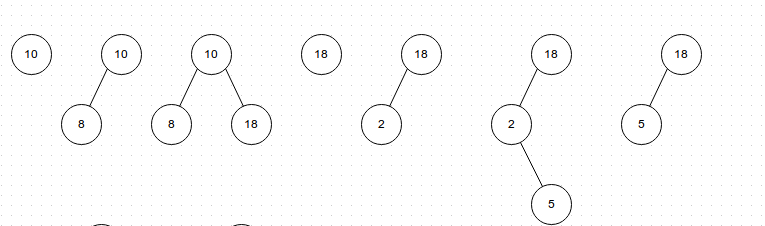
\includegraphics[height=2.0153in,width=6.5972in]{914f4600-1aac-11e3-96b1-99a1a326a3b2.png}

\end{flushleft}


\begin{flushleft}
Starting from the rightmost element, $a_j$ here 10, generate a graph and add 10 as the starting node.
\end{flushleft}


\begin{flushleft}

\end{flushleft}


\begin{flushleft}
	Now traverse the sequence one by one starting from $a_{j-1}$ which is 8.
\end{flushleft}


\begin{flushleft}
	Add 8 to the left of the graph as it is lower than 10.
\end{flushleft}


\begin{flushleft}
	Similarly traverse 8 and add it to the left of the node 10.
\end{flushleft}


\begin{flushleft}
	Here, as 18 is greater than 10 and 8, we will denote the PLE's for 10 and 8 as 18. 
\end{flushleft}


\begin{flushleft}
	And we will remove 10 and 8 from the graph and replace 18 at 10{`}s position.
\end{flushleft}


\begin{flushleft}
	Similarly we will add 2 to the left side of 18 and 5 on the right side of 2.
\end{flushleft}


\begin{flushleft}
	will now replace 2 and the value for 2{`}s PLE will be set as 5.
\end{flushleft}


\begin{flushleft}
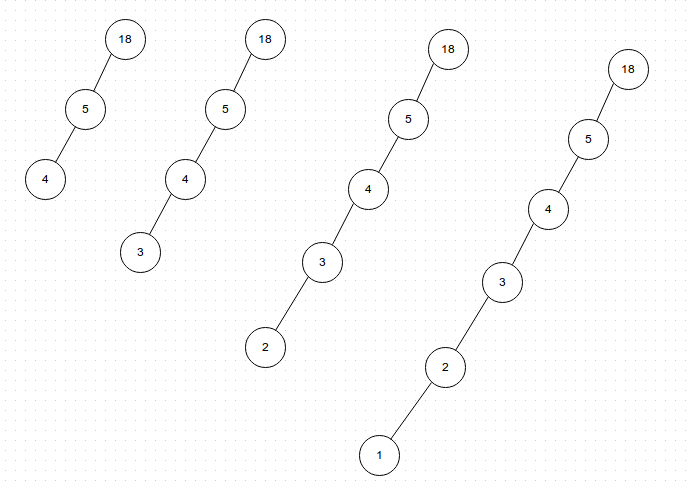
\includegraphics[height=4.0056in,width=6.5125in]{0b338ae4-1aad-11e3-96b1-99a1a326a3b2.png}

\end{flushleft}


\begin{flushleft}
	
\end{flushleft}


\begin{flushleft}

\end{flushleft}


\begin{flushleft}
	Further, add 4,3,2 and 1 each on the left hand side in consecutive steps.\newpage

\end{flushleft}


\begin{flushleft}
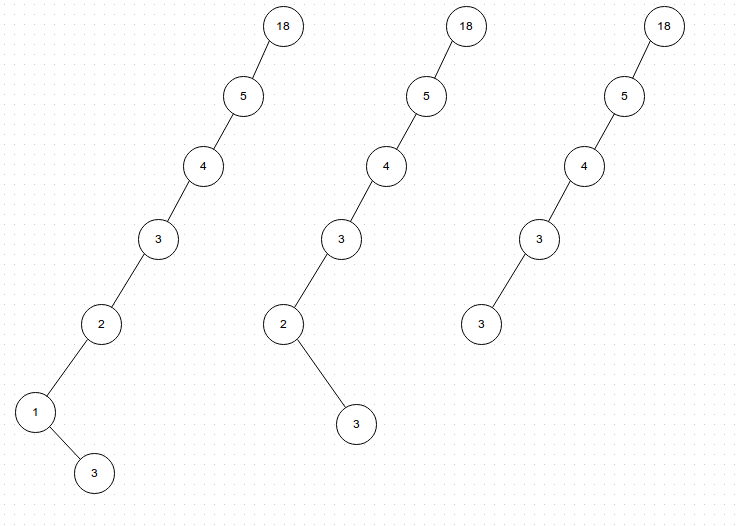
\includegraphics[height=4.8097in,width=6.3514in]{3eca3e60-1aae-11e3-8e67-99a1a326a3b2.png}

\end{flushleft}


\begin{flushleft}
	when 3 is encountered, it will be placed on the right hand side of 1.
\end{flushleft}


\begin{flushleft}
	Now we will denote the PLE for 1 as 3 and replace it in the tree, also as it is greater than 2, it will be placed at the right hand side of 2.
\end{flushleft}


\begin{flushleft}
	Again, 2 will be removed from the tree and 3 will replace its position, PLE of 2 is 3.
\end{flushleft}


\begin{flushleft}
	Now traverse the next number which is 2 and place it on the left hand side of 3.
\end{flushleft}


\begin{flushleft}
	Next traverse the final element, which will remove 2,3,3,4,5 from the graph and mark their PLE's as 6.
\end{flushleft}


\begin{flushleft}

\end{flushleft}


\begin{flushleft}
In the final step, mark PLE's of all the elements still present in the tree as 0.
\end{flushleft}


\begin{flushleft}

\end{flushleft}


\begin{flushleft}
	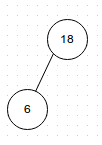
\includegraphics[height=1.51in,width=1.06in]{7d2e89d6-1aae-11e3-8e67-99a1a326a3b2.png}

\end{flushleft}


\begin{flushleft}

\end{flushleft}


\begin{flushleft}

\end{flushleft}


\begin{flushleft}

\end{flushleft}


\begin{flushleft}
\textbf{Problem 4:}
\end{flushleft}


\begin{flushleft}
\textbf{	}\textbf{Given n unsorted numbers, compute the maximum and minimum using $\lceil 3n/2 \rceil -2 $ comparisons.}
\end{flushleft}


\begin{flushleft}

\end{flushleft}


\begin{flushleft}
Solution:
\end{flushleft}


\begin{flushleft}

\end{flushleft}


\begin{flushleft}
The algorithm to compute the maximum and minimum on n elements in $ \lceil 3n/2 \rceil$ 2 comparisons can be done as follows :
\end{flushleft}


\begin{flushleft}

\end{flushleft}


\begin{flushleft}
Step -1 :
\end{flushleft}


\begin{flushleft}
Compare each of the even numbered element with the consecutive element in the list and determine the one that is greater. Add the elements that are larger in a set and name it SET A and the ones that are smaller in another SET B.
\end{flushleft}


\begin{flushleft}

\end{flushleft}


\begin{flushleft}
Step -2 :
\end{flushleft}


\begin{flushleft}
For each element in SET A find the maximum by performing a linear search.
\end{flushleft}


\begin{flushleft}

\end{flushleft}


\begin{flushleft}
Step - 3:
\end{flushleft}


\begin{flushleft}
For each element in SET B find the minimum by performing a linear search.
\end{flushleft}


\begin{flushleft}

\end{flushleft}


\begin{flushleft}
At the end of the algorithm, we will be able to determine the maximum and minimum from a given set of n numbers.
\end{flushleft}


\begin{flushleft}

\end{flushleft}


\begin{flushleft}
Calculating the number of comparisons made in each step of the algorithm:
\end{flushleft}


\begin{flushleft}

\end{flushleft}


\begin{flushleft}
Step -1 : For a given set of n numbers in order to generate two sets for larger and smaller numbers, one needs to make $\lceil n/2\rceil $ Comparisons.
\end{flushleft}


\begin{flushleft}

\end{flushleft}


\begin{flushleft}
Step -2 :  In order to find the maximum from SET A using linear searching technique, one needs to perform, $ \lceil n/2 \rceil-1 $ comparisons. This is because, the number of elements in the set is $ \lceil n/2 \rceil$. So, the number of comparisons required is one less than the total number of elements in the set.
\end{flushleft}


\begin{flushleft}

\end{flushleft}


\begin{flushleft}
Step -3 :  In order to find the minimum from SET B using linear searching technique, one needs to perform, $ \lceil n/2 \rceil $-1 comparisons. This is because, the number of elements in the set is $ \lceil n/2 \rceil $. So, the number of comparisons required is one less than the total number of elements in the set.
\end{flushleft}


\begin{flushleft}

\end{flushleft}


\begin{flushleft}
Hence, total number of comparisons is  $ \lceil n/2 \rceil $ + $ \lceil n/2 \rceil $ -1 +  $ \lceil n/2 \rceil $ -1 
\end{flushleft}


\begin{flushleft}
= 3 $ \lceil n/2 \rceil $-2
\end{flushleft}


\begin{flushleft}
= $ \lceil 3n/2 \rceil $2
\end{flushleft}


\begin{flushleft}
 
\end{flushleft}


\begin{flushleft}
Hence, proved.
\end{flushleft}


\begin{flushleft}

\end{flushleft}


\begin{flushleft}

\end{flushleft}


\begin{flushleft}
 
\end{flushleft}


\begin{flushleft}

\end{flushleft}


\begin{flushleft}

\end{flushleft}


\begin{flushleft}

\end{flushleft}


\begin{flushleft}

\end{flushleft}


\begin{flushleft}
\textbf{Problem 5:}
\end{flushleft}


\begin{flushleft}
\textbf{Page 107 Problem \#4 :}
\end{flushleft}


\begin{flushleft}
	Considering n specimens and collection of m judgments for the pairs that were not declared ambiguous, the algorithm for the problem can be written as:
\end{flushleft}


\begin{flushleft}

\end{flushleft}


\begin{flushleft}
Create two sets A and B:
\end{flushleft}


\begin{flushleft}
For each pair of specimen (i,j) or (j,i) and its corresponding judgment, perform the following:
\end{flushleft}


\begin{flushleft}
Start from node i, add the node to set A.
\end{flushleft}


\begin{flushleft}

\end{flushleft}


\begin{flushleft}
	--If node j is not present in any of the two sets (i.e. if it isn't already traversed)
\end{flushleft}


\begin{flushleft}
		Judgment = {``}same'' -- ADD node j -- to set A,
\end{flushleft}


\begin{flushleft}
		Otherwise -- ADD node j -- to set B.
\end{flushleft}


\begin{flushleft}
	Continue with pairs that contain either of i or j (Neighbors).
\end{flushleft}


\begin{flushleft}
	
\end{flushleft}


\begin{flushleft}
	--Else
\end{flushleft}


\begin{flushleft}
		If the node is present in the correct set (The set determined from the above if condition), continue with the pairs that contain either of i or j (Neighbors).
\end{flushleft}


\begin{flushleft}
		else
\end{flushleft}


\begin{flushleft}
			break and mark the judgment to be inconsistent.
\end{flushleft}


\begin{flushleft}

\end{flushleft}


\begin{flushleft}

\end{flushleft}


\begin{flushleft}
The judgments are consistent if the algorithm exits normally.
\end{flushleft}


\begin{flushleft}

\end{flushleft}


\begin{flushleft}
Running Time: 
\end{flushleft}


\begin{flushleft}
	This algorithm is a slightly modified version of Breadth first Search and hence its running time is $O(|m|+|n|)$ where m is the number of judgments and n is the number of specimens.
\end{flushleft}


\begin{flushleft}

\end{flushleft}


\begin{flushleft}

\end{flushleft}


\begin{flushleft}
\textbf{Page 107 Problem \#6 :}
\end{flushleft}


\begin{flushleft}

\end{flushleft}


\begin{flushleft}
Considering Graph G=(V,E) and Tree T for the below proof.
\end{flushleft}


\begin{flushleft}

\end{flushleft}


\begin{flushleft}
In a BFS tree, the edges of the graph G that appear in tree are either connected in the same layer or to adjacent layer.
\end{flushleft}


\begin{flushleft}

\end{flushleft}


\begin{flushleft}
So based on this property the graph can contain two types of edges, either in the same or in adjacent layers.
\end{flushleft}


\begin{flushleft}

\end{flushleft}


\begin{flushleft}
But, as this tree is also a DFS tree, the property that for any nodes x and y in the tree, either x or y is an ancestor of the other prevails.
\end{flushleft}


\begin{flushleft}

\end{flushleft}


\begin{flushleft}
Hence only one type of edges are present and they are only between adjacent layers.
\end{flushleft}


\begin{flushleft}

\end{flushleft}


\begin{flushleft}
This proves the fact that there cannot be any other types of edges in T and hence no extra edges are present in G.
\end{flushleft}


\begin{flushleft}

\end{flushleft}


\begin{flushleft}
Hence, proved.
\end{flushleft}


\begin{flushleft}

\end{flushleft}


\begin{flushleft}
\textbf{Page 107 Problem \#10 :}
\end{flushleft}


\begin{flushleft}

\end{flushleft}


\begin{flushleft}
We can apply a slight modification of the BFS Algorithm for this problem.
\end{flushleft}


\begin{flushleft}
The central idea for the algorithm is to maintain a list of reachability information to every node from the starting node and use this information to calculate the number of possible shortest paths.
\end{flushleft}


\begin{flushleft}

\end{flushleft}


\begin{flushleft}
In order to find the number of shortest paths between node(i,j), we will start performing a BFS graph traversal from node i. 
\end{flushleft}


\begin{flushleft}
- We will assign the reachability of node i as 0.
\end{flushleft}


\begin{flushleft}
- From node i, we will assign the reachability as 1 for all the neighbors of i.
\end{flushleft}


\begin{flushleft}
- Similarly we will perform BFS on each of the neighbors of node i and assign their reachability as , 1+ reachability of previous node.
\end{flushleft}


\begin{flushleft}
- We will perform this until all the nodes have been traversed.
\end{flushleft}


\begin{flushleft}

\end{flushleft}


\begin{flushleft}
Once all of this information is gathered, we need to traverse the graph from reverse direction, from node j and count the number of incoming edges that have the lowest reachability number.
\end{flushleft}


\begin{flushleft}

\end{flushleft}


\begin{flushleft}
We need to follow all such edges until node i, and increment the counter every time , if there are more than one edges having same lowest reachability which are incident on a node.
\end{flushleft}


\begin{flushleft}

\end{flushleft}


\begin{flushleft}
The running time for his algorithm is $O(m+n)$ because we are using primarily using BFS for most of the computation. 
\end{flushleft}


\begin{flushleft}

\end{flushleft}


\begin{flushleft}

\end{flushleft}


\begin{flushleft}

\end{flushleft}


\begin{flushleft}

\end{flushleft}


\begin{flushleft}

\end{flushleft}




12
\end{document}
